\chapter{LoRaWAN relay mode}
\label{chap:relayproto}

LoRaWAN networks typically are laid out in a star-of-star topology, in which end-devices communicate directly with one or more gateways, but there are many cases in which it could be useful to have a special node able to act as relay between end-devices and the gateway.

In this chapter an extension to the LoRaWAN protocol is defined, which allows the end-devices to discover and bind to any nearby relay eligible node.


\section{Motivations}

As described in chapter \ref{chap:lorawan}, the LoRaWAN protocol is designed to be deployed in a star-of-star layout, in which all the end-devices need only one LoRa communication to reach the IP network.

This architecture, of course, significantly simplifies the protocol, eliminating the need of routing mechanisms, but, on the other hand, it requires the installation of new gateways to expand the coverage area of the network.

The standard LoRa gateways, in general, require an IP connection to operate as described in the specification, and in some contexts (e.g. rural areas with no cellular coverage) it may be an impossible requirement to satisfy.

On the contrary, the solution proposed in this thesis allows to extend the coverage area without the need of gateways, and, at the same time, to increase the performances of the end-devices at the same range of coverage.


\section{Design}
\label{sec:protdesign}

\subsection{Protocol overview}

\begin{figure}
\centering
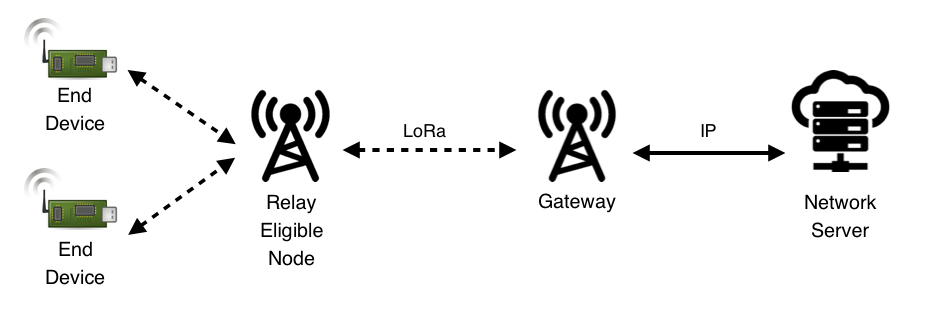
\includegraphics[width=\textwidth]{img/relay-architecture}
\caption{Reference architecture of relay mode}
\label{fig:relayarch}
\end{figure}

The main obstacle to design a relay solution in a LoRaWAN network is that the end-devices which will act as relays often have only one LoRa interface, and also the transceivers installed on these devices are not capable to open receive windows at the same time on all possible frequencies, data rates and coding rates.

With the aim to design a protocol that can be implemented on this type of end-devices it was decided to add a TDMA technique to the standard specification. The key idea is that each \emph{Relay Eligible Node} must periodically send a beacon to advertise itself to nearby end-devices. The interval of time between two beacons sent by the same relay node is called \emph{Beacon Period}. Each beacon period is divided into two different phases:

\begin{itemize}

\item \emph{Bind Phase}, in which end-devices try to bind themselves with the relay node;

\item \emph{Transmission Phase}, in which end-devices send upstream data to relay and receive downstream data.

\end{itemize}
The transmission phase is further divided into several slots, numbered starting from zero, in order to let the relay node wake up only when needed, i.e. only in proximity of slots bound to end-devices.
In each slot only one end-device is allowed to exchange data, and each end-device can transmit only in one slot per beacon period. The slot within the beacon period is assigned to the end-device by the network server in the bind phase. One slot is reserved to bind answers, and it is never assigned to devices.

\begin{figure}
\centering
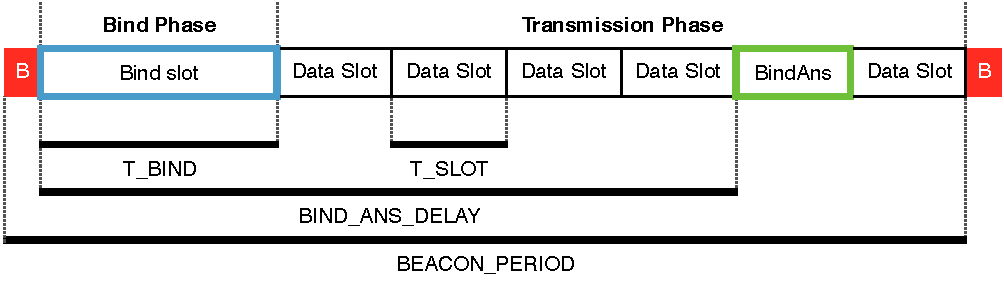
\includegraphics[width=\textwidth]{img/timing_diagram}
\caption{Timing diagram of the protocol}
\label{fig:timepdia}
\end{figure}

The beacons and all bind messages are sent using well known parameters (data rate, coding rate, frequency), which are defined in this specification. The other communications are performed using parameters which must be exchanged in bind phase.

The aim of this protocol is to extend LoRaWAN without radically changing its philosophy, so every decision is taken by the network server, which sets up both the relays and the end-devices through MAC commands.

\paragraph{Requirements} Although the very centralized nature of LoRaWAN is maintained with the new relay mode, this is not transparent to existing devices, which need to be adapted in order to support the new protocol. In particular:

\begin{itemize}
\item The end-devices must explicitly switch to relay mode;
\item The relay node must explicitly switch to relay mode, advertising its presence to neighbors and exchanging all needed parameters with the network server;
\item The network server must be update to support the new mode;
\item End-devices and relay must belong to the same network, such that they are managed by the same network server;
\end{itemize}

On the other hand, existing LoRa gateways already support the new relay mode because they do not interact with the LoRaWAN layer. Furthermore, existing standard LoRaWAN end-devices are not affected by the behavior of the updated devices. 



\paragraph{Specification} This specification includes the format of all newly defined massages and the description of the timing constraints. It can be logically divided into three parts:

\begin{itemize}
\item \emph{Relay eligible node management}: defines all the messages exchanged between the relay and the network server;

\item \emph{End-device binding}: defines all the messages exchanged in order to effectively bind (and unbind) end-devices to the relay;

\item \emph{Data transmission}: defines the protocol to adopt when an end-device wants to transmit upstream data and receive downstream data, if any.
\end{itemize}


\subsection{Relay eligible node management}

\subsubsection{Relay setup}

Before starting to advertise itself, each relay eligible node must send a \emph{RelaySetupReq} MAC command to network server, containing the minimum requirements for the parameters of the relay session.

\begin{figure}[!h]
\centering
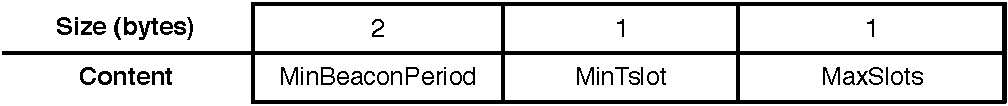
\includegraphics[width=\textwidth]{img/commands/RelaySetupReq}
\caption{RelaySetupReq MAC command}
\label{fig:relaysetupreq}
\end{figure}

In particular MinBeaconPeriod contains the minimum length of the BeaconPeriod expressed in seconds; MinTslot contains the minimum length of the slot expressed in seconds; MaxSlots contains the maximum number of slots per BeaconPeriod which the device is able to handle.

The relay node cannot advertise itself until it receives the parameters from network server through RelaySetupAns MAC command.

\begin{figure}[!h]
\centering
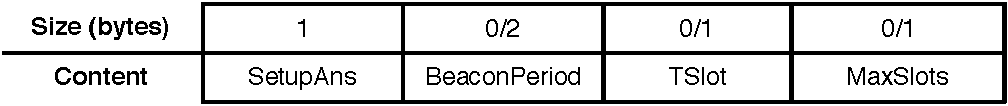
\includegraphics[width=\textwidth]{img/commands/RelaySetupAns}
\caption{RelaySetupReq MAC command}
\label{fig:relaysetupans}
\end{figure}

In particular if SetupAns equals 0x00 the device is accepted, and this field is followed by the mandatory parameters to adopt. The BeaconPeriod and the slot length TSlot are expressed in seconds. MaxSlots is the number of available slots.

If SetupAns is not equal to 0x00 the device was not accept by the network server as a relay, and it is not followed by any other fields.




\subsubsection{Relay status}
The relay may request to the network server the list of end-devices bound to it. In response it will receive the changes on the list of served end-devices from last request.
The \emph{RelayStatusReq} does not have any payload, the \emph{RelayStatusAns} has the format of figure \ref{fig:relaystatusans} and each \emph{DeviceEntry} is encoded as figure \ref{fig:deventry}

\begin{figure}[!h]
\centering
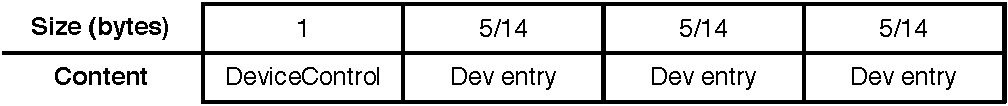
\includegraphics[width=\textwidth]{img/commands/RelayStatusAns}
\caption{RelayStatusAns MAC command}
\label{fig:relaystatusans}
\end{figure}
The \emph{DeviceControl} field (figure \ref{fig:devcontrol}) carries the \emph{ClearList} flag and the number of devices (\emph{DeviceNum}) contained into the following list.  When the \emph{ClearList} flag is set, the end-device must empty its current list before updating it with the new information contained in this MAC command.

\begin{figure}[!h]
\centering
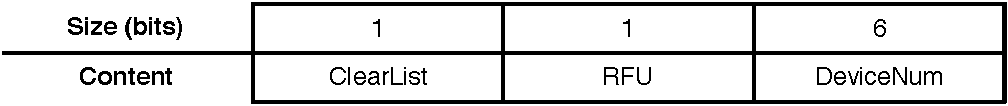
\includegraphics[width=\textwidth]{img/commands/DeviceControl}
\caption{DeviceControl field in the RelayStatusAns MAC command}
\label{fig:devcontrol}
\end{figure}

\begin{figure}[!h]
\centering
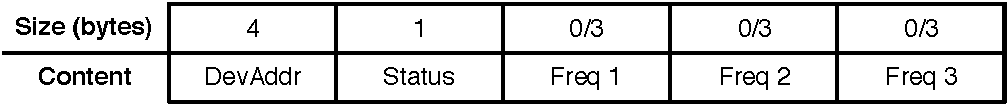
\includegraphics[width=\textwidth]{img/commands/DevEntry}
\caption{Device entry contained in RelayStatusAns MAC command}
\label{fig:deventry}
\end{figure}
The RelayStatusAns can carry as many device entry as they fit in the packet, with an upper bound of 63. Each device entry contains the address (DevAddr) and the Status of the device, which has the format described in figure \ref{fig:deventrystatus}.

\begin{figure}[!h]
\centering
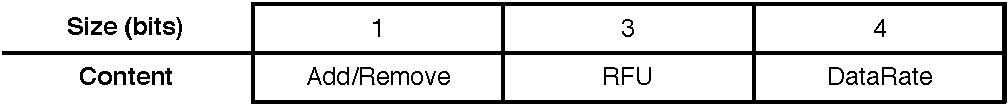
\includegraphics[width=\textwidth]{img/commands/DevEntryStatus}
\caption{Status fiend within each device entry}
\label{fig:deventrystatus}
\end{figure}

If the Add/Remove flag is set, then the relay must deallocate the slot for the end-device. Else if the Add/Remove flag is not set, then the DataRate field carries the data rate at which the end-device will transmit its messages, and the Status field is followed by 9 octets carrying the three frequencies on which the end-device will transmit.

\subsubsection{Relay stop}
The network server can stop a relay node using the \emph{RelayStopReq} MAC command. When the relay node receives the RelayStopReq command it must stop every relay activity immediately, hence the network server does not expect any answer. This command does not have any payload.


\subsection{End-device binding}
\begin{figure}[]
\centering
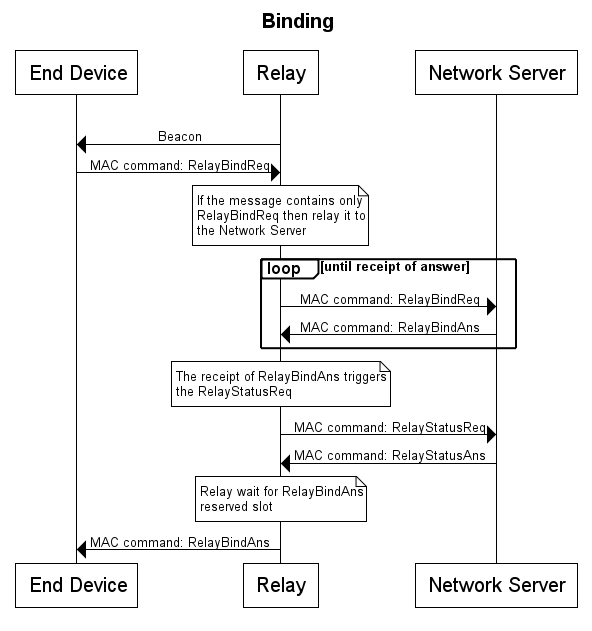
\includegraphics[width=\textwidth]{img/seqdia/binding}
\caption{Sequence diagram of the end-device binding}
\label{fig:binding}
\end{figure}

In order to bind to a relay node, the end-device starts listening to the radio channel, waiting for a beacon. If the end-device receives a beacon from a relay node it can decide either to bind to it by sending a \emph{RelayBindReq} command, or to discard the beacon and start waiting for a new one.


\subsubsection{Broadcasting Beacons}

In order to advertise its presence to its neighbors, the relay node periodically sends a beacon containing all the information needed by end-devices to set up a session with it. The beacon must be sent with the parameters reported in table \ref{tab:beaconparams}.


% Please add the following required packages to your document preamble:
% \usepackage{booktabs}
\begin{table}[]
\centering
\caption{Transmission parameters of the beacon}
\label{tab:beaconparams}
\begin{tabular}{@{}ll@{}}
\toprule
\multicolumn{1}{c}{Parameter} & \multicolumn{1}{c}{Value} \\ \midrule
Data Rate                     & SF9 BW125                 \\
Coding Rate                   & 4/5                       \\
Frequency                     & 869.525 MHz               \\
Period                        & BEACON\_PERIOD            \\ \bottomrule
\end{tabular}
\end{table}



\begin{figure}[!h]
\centering
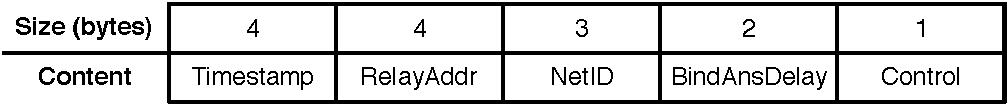
\includegraphics[width=\textwidth]{img/Beacon}
\caption{Beacon format}
\label{fig:beacon}
\end{figure}


Relay must include in the beacon its address (RelayAddr) and the ID of the network (NetID) to which it belongs to, in order to let the end-device select only relays belonging to its own network. The NetID has the format described in the LoRaWAN specifications. The Timestamp field contains the internal timestamp of the relay node, using milliseconds unit of measure. The Control field contains RFU flags.



\subsubsection{RelayBindReq}

The bind request must be sent only in the bind slot, and exactly RX\_DELAY seconds after the end of the beacon transmission. The bind request must be performed using MAC command RelayBindReq, which has the format shown in figure \ref{fig:relaybindreq}.

\begin{figure}[!h]
\centering
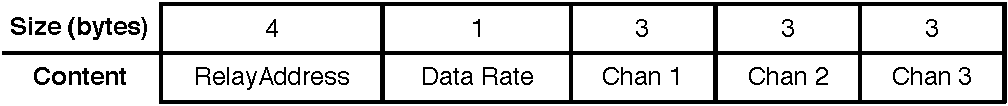
\includegraphics[width=\textwidth]{img/commands/RelayBindReq}
\caption{RelayBindReq MAC command}
\label{fig:relaybindreq}
\end{figure}

These parameters are used by the relay to open the receive window at the beginning of the transmission slot. Each \emph{Chan} field contains the center frequency of the channel, expressed in Hertz and divided by 100. For instance, if the center frequency of the channel is 868300000 Hz, the corresponding \emph{Chan} field into the RelayBindReq will contain the number 8683000.

The \emph{DataRate} field is encoded as shown in figure \ref{fig:datarate}.

\begin{figure}[!h]
\centering
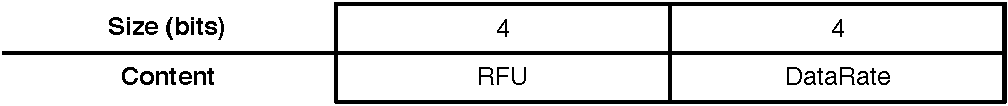
\includegraphics[width=\textwidth]{img/commands/DataRate}
\caption{DataRate field into RelayBindReq MAC command}
\label{fig:datarate}
\end{figure}

\subsubsection{RelayBindAns}
Network server must answer to a RelayBindReq with a RelayBindAns MAC command, which has the format shown in figure \ref{fig:relaybindans}.

\begin{figure}[!h]
\centering
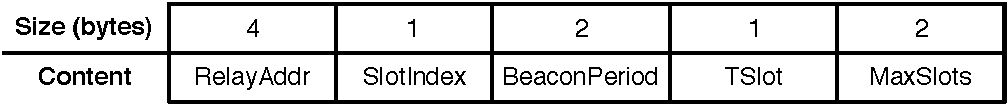
\includegraphics[width=\textwidth]{img/commands/RelayBindAns}
\caption{RelayBindAns MAC command}
\label{fig:relaybindans}
\end{figure}

The recipient of a RelayBindAns MAC command is the end-device who has sent the RelayBindReq. The network server must include in the RelayBindAns MAC command the following information:

\begin{description}
\item[RelayAddr] the address of the relay;
\item[SlotIndex] index of the time slot assigned to the device;
\item[BeaconPeriod] time-interval between two beacons, expressed in seconds;
\item[TSlot] time slot length, expressed in seconds;
\item[MaxSlots] number of slots within one beacon period.
\end{description}
The end-device will receive the RelayBindAns MAC command into the \emph{BindAns} slot, which is advertised within the beacon through the field \emph{BindAnsDelay}. If the RelayBindAns MAC command is not received in the first available BindAns slot, the original RelayBindReq must be considered lost and the end-device must perform a new bind request.

\subsubsection{RelayUnbindReq}

\begin{figure}[!h]
\centering
\includegraphics[width=\textwidth]{img/seqdia/unbinding}
\caption{Sequence diagram of the end-device unbinding}
\label{fig:unbinding}
\end{figure}

The end-device may explicitly unbind from its relay by sending a \emph{RelayUnbindReq} MAC command to the network server, which reacts de-allocating the time slot reserved to the end-device starting from the next beacon period. The RelayUnbindReq contains only the command identifier without parameters.

The network server may also autonomously detect the unbinding of the end-device, considering the device unbound after \emph{MAX\_EMPTY\_SLOTS} slots without receiving data from the end-device. So, in order to keep the session alive, the end-device must send an upstream message at least every MAX\_EMPTY\_SLOTS / 2 slots.

The end-device may use the the \emph{LinkCheckReq} MAC command to detect the unbinding. If after \emph{MAX\_LINK\_CHECK\_REQUESTS} the end-device does not receive any \emph{LinkCheckAns}, it considers itself unbound.




\subsection{Data transmission}
Each client is allowed to send upstream messages only within its own slot, using the previously agreed channel parameters.

\begin{figure}[]
\centering
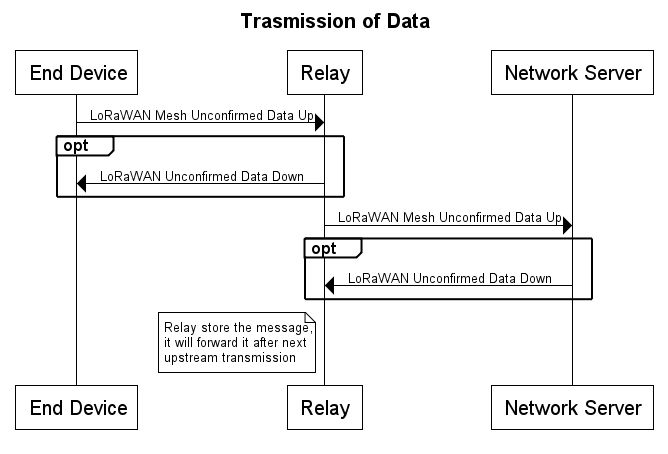
\includegraphics[width=\textwidth]{img/seqdia/datatx}
\caption{Sequence diagram of the data transmission}
\label{fig:datatx}
\end{figure}



\subsubsection{Communication between end-device and relay}
\paragraph{Channel selection}
During bind phase the client node must include into the \emph{RelayBindReq} command three channel definitions to use in transmission phase. Both the client and the relay must cycle on list of channels in the order they are defined in the \emph{RelayBindReq}, so at the first available slot after binding both devices must use the first channel defined, then they must loop on the list of channels. 

\paragraph{Message type}
Each end-device operating in relay mode must tag its messages in order to let the network server distinguish between directly sent messages and relayed ones. This can be done introducing new message type called \emph{Mesh Unconfirmed Data Up} (type 110). 
All upstream messages sent by an end-device will have Mesh Unconfirmed Data Up as type, and they will not be acknowledged by the network server.
When a network server receive a Mesh Unconfirmed Data Up message, it should discard all the statistics collected by the gateway (e.g. RSSI) because the device who has transmitted the message to the gateway, i.e. relay, is not the device indicated in the DevAddress field, i.e. the end-device.


\subsubsection{Communication between relay and gateway}
The communication between the relay node and the gateway follows the LoRaWAN 1.0 specification, except for the fact that all upstream message have the newly defined Mesh Unconfirmed Data Up as message type.
Given that relay forwards exactly the LoRaWAN message it has received, it may receive an answer form the network server which will have ClientAddr as DestAddr. The relay node must store the message until next transmission form the end-device, than it must forward it.


\subsection{MAC Commands and parameters}
As already stated, all the set up information between end-devices, relay and network server are exchanged by means of MAC commands. The new MAC commands defined in this protocol are summarized in table \ref{tab:commands}.

% Please add the following required packages to your document preamble:
% \usepackage{booktabs}
% \usepackage{multirow}
\begin{table}[]
\centering
\caption{MAC commends}
\label{tab:commands}
\begin{tabular}{@{}llcccl@{}}
\toprule
\multicolumn{1}{c}{\multirow{2}{*}{CID}} & \multicolumn{1}{c}{\multirow{2}{*}{Command}} & \multicolumn{3}{c}{Transmitted by} & \multicolumn{1}{c}{\multirow{2}{*}{Description}}                                                                               \\
\multicolumn{1}{c}{}                     & \multicolumn{1}{c}{}                         & ED        & Relay       & NS       & \multicolumn{1}{c}{}                                                                                                           \\ \midrule
0x80                                     & RelaySetupReq                                &           & x           &          & \begin{tabular}[c]{@{}l@{}}Requests parameters to start\\ acting as a relay, attaching\\ the minimum requirements\end{tabular} \\ \midrule
0x81                                     & RelaySetupAns                                &           &             & x        & \begin{tabular}[c]{@{}l@{}}Answer to RelaySetupReq,\\ with the requested parameters\end{tabular}                               \\ \midrule
0x82                                     & RelayStatusReq                               &           & x           &          & \begin{tabular}[c]{@{}l@{}}Requests the network server\\ to send changes on bound\\ end-devices\end{tabular}                   \\ \midrule
0x83                                     & RelayStatusAns                               &           &             & x        & \begin{tabular}[c]{@{}l@{}}List of new end-devices or\\ “clear list” command\end{tabular}                                      \\ \midrule
0x84                                     & RelayStopReq                                 &           &             & x        & Requests the relay to stop                                                                                                     \\ \midrule
0x85                                     & RelayBindReq                                 & x         &             &          & Requests to bind to a relay                                                                                                    \\ \midrule
0x86                                     & RelayBindAns                                 &           &             & x        & Answer to RelayBindReq                                                                                                         \\ \midrule
0x87                                     & RelayUnbindReq                               & x         &             &          & \begin{tabular}[c]{@{}l@{}}Notifies the network server\\ the unbinding of an end-device\end{tabular}                           \\ \bottomrule
\end{tabular}
\end{table}


The value of each parameter is not fixed into the specification, but it can be determined upon installation according to the use case. In table \ref{tab:params} there are some tested parameters.


% Please add the following required packages to your document preamble:
% \usepackage{booktabs}
\begin{table}[]
\centering
\caption{Parameters}
\label{tab:params}
\begin{tabular}{@{}ll@{}}
\toprule
\multicolumn{1}{c}{Constant} & \multicolumn{1}{c}{Value} \\ \midrule
BEACON\_PERIOD               & 300 s                     \\
RX\_DELAY                    & 1 s                       \\
MAX\_LINK\_CHECK\_REQUESTS   & 10                        \\
MAX\_EMPTY\_SLOTS            & 20                        \\
T\_BIND                      & 30 s                      \\
T\_SLOT                      & 10 s                      \\
MAX\_SLOTS                   & 28                        \\ \bottomrule
\end{tabular}
\end{table}






\section{Implementation}

The \emph{Waspmote Pro} is a model of mote produced by Libelium and designed for the Internet of Things. It consists of a small board which includes an ATmega 1281 microcontroller, some analog and digital I/O pins, one socket for the GPS module and two sockets for the radio modules. The latter can be used to install on the Waspmote Pro transceivers for different radio technologies like Zigbee, Wi-Fi, Sigfox and LoRaWAN.

Each transceiver implements in hardware the network protocol for which it was designed, and it gives access to its features through a limited set of APIs. The philosophy behind these design choices is that the transceiver is responsible for the correct implementation of the network protocol, especially for the timing constraints, so each update of the network protocol involves the redesign of the radio module.

Since there was not the possibility of producing a new transceiver updated to the specifications described in section \ref{sec:protdesign}, it was decided to implement a subset of the protocol in software, introducing minor changes in order to overcome the inability to operate directly at the physical level.

In particular, the limitations of the platform that do not allow the full implementation of the protocol in software are the following:

\begin{itemize}
\item Single thread programming: the standard Waspmote Pro SDK does not allow to create multi-thread applications;

\item Granularity of power saving mode: the APIs allow to enter power saving mode with the granularity of seconds, so to have more precision it is necessary to use busy wait;

\item Impossibility to synchronize the internal clock with other motes without using the GPS module;

\item Synchronous APIs with varying lengths of time between send and receive calls. Since the synchronization between two nodes is done taking as reference point the instant at which ends the transmission of a message, every inaccuracy on the duration of the API call must be properly handled; 

\item Limited amount of memory: RAM and ROM are limited respectively to 8 Kb and 128 Kb;

\item Limitations of high-level LoRaWAN API: using such API is impossible to modify fields into the LoRaWAN message other than \emph{FPort} and \emph{FPayload}, so every modification must be emulated carrying some additional information into the payload.
\end{itemize}


\subsection{Assumptions}
Given all the limitations previously described, it has been decided to implement only the transmission phase, considering all the end-devices already bound to the relay node.

For testing purposes all the information normally exchanged during the RelaySetup and the RelayBind phases were statically pre-loaded on the devices. Summarizing, once an end-device has booted up, the operations it must perform are the following:
\begin{enumerate}
\item It must wait for a beacon from the relay node in order to synchronize its reference time with it;
\item It must transmit the data exactly at the beginning of its transmission slot. 
\end{enumerate}
Potential differences of the internal clock must be taken into account by the relay node opening the receive windows slightly before the beginning of the slot, and keeping it open for a sufficient\footnote{In an hardware implementation with precise timing the minimum length of the receive window can be reduced to the time needed to identify the preamble of the LoRa physical frame, but in a software implementation the interval of time must to be larger in order to overcome the impossibility to operate at the physical layer. Moreover the exact waiting time must be evaluated experimentally since it depends on the platform used.} interval of time.

Regarding the implementation of the relay, since it is assumed that there is no bind phase, every \texttt{BEACON\_PERIOD} it must:
\begin{enumerate}
\item broadcast the beacon on the predefined channel, without opening the receive windows normally used to detect bind requests;
\item for each slot, open the receive window; in case of receipt of data send to the end-device any cached message, and forward  the data to the gateway as soon as possible.
\end{enumerate}
Table \ref{tab:relayparams} reports the parameters used for the implementation.

% Please add the following required packages to your document preamble:
% \usepackage{booktabs}
\begin{table}[]
\centering
\caption{Parameters of the relay mode}
\label{tab:relayparams}
\begin{tabular}{@{}ll@{}}
\toprule
Constant       & Value \\ \midrule
BEACON\_PERIOD & 35 s  \\
RX\_DELAY      & 1 s   \\
T\_BIND        & 5 s   \\
T\_SLOT        & 15 s  \\
MAX\_SLOTS     & 2     \\ \bottomrule
\end{tabular}
\end{table}


\subsection{End-device}
\label{subsec:enddev}

Due to the timing constraints of the LoRaWAN APIs, every transmission between the end-device and the relay must be performed using the LoRa P2P APIs\footnote{Also indicated as "Direct communications between nodes" in the "Waspmote LoRaWAN networking guide"} provided by Libelium. \cite{waspmote}

The new \emph{Mesh Unconfirmed Data Up} message type is implemented directly into the MAC header, and the whole LoRaWAN packet is built by the mote, in contrast with standard LoRAWAN communications where the transceiver is in charge to build the packet.

As result of this architecture the computation of the MIC for each message should be performed on the mote, which is not possible due to the lack of stable implementation of the security algorithms needed for this purpose. For these reasons, and only in test environment, it has been decided to not attach the MIC field to the packet.

On the contrary, the encryption of the Frame Payload is technically possible with the standard Waspmote libraries, but it has been decided to not perform it since it is not essential for the experimentation purposes.


\subsubsection{Implementation on Waspmote Pro}
At the start up the end-device has to switch on the radio module and set up all the needed parameters, which are pre-loaded on the board.

Then, before sending any upstream data, the end-device must synchronize itself with relay by means of the beacon, and, as it is shown in listing \ref{list:enddev}, this operation is done by calling the function \texttt{waitForBeacon()}. The \texttt{waitForBeacon()} function returns the time stamp at which the beacon is received (or zero if any error has occurred), which is used as reference time to compute the beginning of the following slots.

After the synchronization through the beacon, the end-device switch to the pre-configured parameters for data transmission and pauses until the beginning of its own slot. Then, it sends the upstream data, and after \texttt{RX\_DELAY - T\_TOLERANCE} milliseconds opens the receive windows with exactly the same configuration as the uplink transmission. The receive window is opened 	\texttt{T\_TOLERANCE} milliseconds before actual beginning in order to overcome to possible differences with the relay internal clock, and to compensate it is kept open for \texttt{RX\_WINDOW + T\_TOLERANCE} millisecond.

At the end of receive window if something has been received it is shown on the serial monitor, then the frame counter is incremented and the end-device pauses for a \texttt{PERIOD} until next transmission slot is available.

\begin{lstlisting}[caption=Implementation of the end-device\label{list:enddev}]
void loop() {
  uint32_t start = waitForBeacon();
  if (start == 0) {
    return;
  }

  configureRadio(tx_freq,tx_sf);
  waiting_time = start + T_BIND - millis() + (slot*T_SLOT);
  if (waiting_time > 0) {
    delay(waiting_time);
  } else {
    return;
  }

  // Send  data
  while (1) {
    timestamp = millis();
    error = upMessage.sendFrame();
    uint32_t end_tx = millis();

    if (error == 0) {
      USB.println(F("--> Packet sent"));

      // Receive answer
      waiting_time = RX_DELAY - (millis() - end_tx) - T_TOLERANCE;
      if (waiting_time > 0) {
        delay(waiting_time);
      } else {
      	return;
      }
      error = downMessage.receiveFrame(RX_WINDOW + T_TOLERANCE);

      if (error == 0) {
        USB.print(F("--> Packet received: "));
        USB.println(downMessage.getBuffer());
      } else if (error == 2) {
        USB.println(F("--> Timeout! No packet received"));
      } else {
        USB.println(F("Error receiving packet"));
      }
    }
    else {
      USB.println(F("Error sending packet"));
    }

    // Update frame counter
    upMessage.setFrameHeader(DEVICE_ADDR, ++counter_up);
    upMessage.setMessage(1, payload);

    waiting_time = PERIOD - (millis() - timestamp);
    if (waiting_time > 0) {
      delay(waiting_time);
    } else {
      return;
    }
  }
}
\end{lstlisting}
As stated before, the synchronization with the relay is done by means of the \texttt{waitForBeacon()} function, which is reported in listing \ref{list:waitforbeacon}. The implementation is pretty straightforward since it just switch to the frequency and spreading factor on which the beacon is sent and wait for it for at most \texttt{PERIOD + T\_TOLERANCE}. If a beacon is detected it return the instant of time at which the transmission ended (plus the overhead of the API, which is taken into account through the \texttt{T\_TOLERANCE} delay), otherwise it returns 0.

\begin{lstlisting}[caption=Wait for beacon on the end-device\label{list:waitforbeacon}]
uint32_t waitForBeacon() {
  Utils.setLED(LED0, LED_ON);
  configureRadio(beacon_freq, beacon_sf); // 869.525 MHz, SF 9
  USB.println(F("--> Waiting for beacon"));
  error = LoRaWAN.receiveRadio(PERIOD + T_TOLERANCE);
  uint32_t start = millis();

  if (error == 0) {
    USB.print(F("beacon: "));
    USB.println((char*) LoRaWAN._buffer);
    waiting_time = RX_DELAY - (millis() - start);
    if (waiting_time > 0) {
      delay(waiting_time);
    }
  } else if (error == 2) {
    USB.println(F("No beacon found"));  
    return 0;
  } else {
    USB.println(F("Error waiting for beacon"));
    return 0;
  }
  Utils.setLED(LED0, LED_OFF);
  return start;
}
\end{lstlisting}

\subsection{Relay}

Since the implementation of the protocol does not include the \emph{Bind Phase}, the behavior of the relay node is slightly different from the specifications.

\paragraph{Bind Slot} Exactly at the beginning of the slot the relay node broadcasts its beacon, using format and parameters described in section \ref{sec:protdesign}. Since the Bind Phase is not implemented the receive window after it is not opened.

\paragraph{Transmission Slots} Exactly RX\_TOLERANCE milliseconds before the beginning of each slot the relay node opens its receive windows with parameters (data rate and frequency) defined for the end-device to which the slot is assigned. If the relay receives data, it performs the following operations:

\begin{enumerate}
\item if there is a pending packet to be relayed to the end-device, it sends it following the specifications detailed in chapter \ref{chap:relayproto}, except for the MIC as explained in \ref{subsec:enddev};
\item the relay switches to the LoRaWAN APIs;
\item it sets up the LoRaWAN module with the parameters (address, keys, counters) of the end-device from which it has received data;
\item the relay forwards the received data to the gateway;
\item it automatically opens the two LoRaWAN receive windows, and if it receives a packet it is stored in a dedicated buffer, waiting to be relayed after next end-device transmission.
\end{enumerate}

\subsubsection{Implementation on Waspmote Pro}
Once the relay has booted up it must switch on the LoRaWAN module and configure it. The information about the beacon broadcasting and the transmission slot of the end-devices are pre-loaded on the board.

After the initial setup, the relay node performs and infinite loop (reported in listing \ref{list:relay}) in which it broadcasts the beacon and then it opens the receive window at the beginning of the slot of each end-device. 

The beacon broadcasting is done by means of the \texttt{sendBeacon()} function, which returns the time stamp corresponding at the end of transmission, plus the API overhead. As for the end-device, also int this case the time stamp is uses for the timing of the following transmission slots.

Then, \texttt{T\_TOLERANCE} milliseconds before the beginning of each slot the receive window is opened for \texttt{RX\_WINDOW + T\_TOLERANCE} milliseconds. As for the end-device, \texttt{T\_TOLERANCE} is used in order to overcome to possibly de-synchronizations. Moreover, since no bind operation is performed, there no way for the relay to know whether the end-device is active and synchronized with it or not, so in this static implementation the relay must open the receive window for all the end-devices in its internal list.

If the relay receives something from and end-device, it sends back the cached downstream message to it (if present). Then it forwards the end-device upstream message to the gateway by means of the \texttt{forwardMessage()} function, which is reported in listing \ref{list:forward}.


\begin{lstlisting}[caption=Implementation of the relay\label{list:relay}]
void loop() {
  uint32_t beaconTime = millis();
  uint32_t start = sendBeacon() + T_BIND;
  uint8_t slot = 0;

  do {
    Device &client = devices[slot];
    if (configureRadio(client.frequency, client.sf) == 0) {
      waiting_time = start - millis() + (slot*T_SLOT) - T_TOLERANCE;
      if (waiting_time > 0) {
        delay(waiting_time); // Wait for transmission slot
      } else {
        USB.println(F("Time overflow waiting for slot"));
        slot++;
        continue;
      }

      Utils.setLED(LED1, LED_ON);
      error = LoRaWAN.receiveRadio(RX_WINDOW + T_TOLERANCE);
      uint32_t rx_time = millis();
      if (error == 0) {
        client.upMsg.parse((char*) LoRaWAN._buffer); // save up data
        if (client.messagePending) { // forward down data
          waiting_time = rx_time + RX_DELAY - millis();
          if (waiting_time > 0) {
            delay(waiting_time);
            error = client.downMsg.sendFrame(client.frequency); 
            if (error != 0) {
              USB.print(F("Error sending msg to device. error = "));  
              USB.println(error, DEC);
            }
            client.messagePending = false;
          }
        }
        forwardMessage(client); // forward up data to gateway
      } else if (error == 2) {
        USB.print(F("No packet received in slot = "));
        USB.println(slot, DEC);
      } else {
        USB.println(F("Error waiting for packets"));
      }
      Utils.setLED(LED1, LED_OFF);
    } else {
      USB.println(F("Error radio configuration"));
    }
    slot++;
  } while (slot < MAX_SLOTS);

  if (configureRadio(frequency, spreading_factor) != 0) {
    USB.print(F("Set Radio Frequency error = "));
    USB.println(error, DEC);
  }
  
  waiting_time = PERIOD - (millis() - beaconTime);
  if (waiting_time > 0) {
    delay(waiting_time); // Wait for next beacon
  } else {
    USB.println(F("Time overflow waiting for beacon"));
  }
}
\end{lstlisting}
Listing \ref{list:sendbeacon} shows the \texttt{sendBeacon()} function, which just sends the beacon and returns the time stamp.
\\
\begin{lstlisting}[caption=Broadcasting beacon to nearby end-devices\label{list:sendbeacon}]
uint32_t sendBeacon() {
  Utils.setLED(LED0, LED_ON); // Sets the red LED ON
  createBeacon(beacon_buffer);
  error = LoRaWAN.sendRadio(beacon_buffer);
  uint32_t start = millis();
  if (error == 0) {
    USB.println(F("--> Beacon sent"));
  } else {
    USB.print(F("Error sending beacon. error = "));  
    USB.println(error, DEC);   
  }
  Utils.setLED(LED0, LED_OFF); // Sets the red LED OFF
  return start;
}
\end{lstlisting}

The operation of relaying messages to the gateway is done using the \texttt{forwardMessage()} function, reported in listing \ref{list:forward}. Since the communication between relay and gateway is done by means of the high level LoRaWAN APIs, this function is responsible for switching on the LoRaWAN layer on the radio module and send the data. The LoRaWAN layer must be configured with address and keys of the end-device, so that the message can be correctly authenticated and dencrypted by the server.

In this phse the relay may also receive one downstream message addressed to the end-device, which is cached and forwarded to it the next time the end-device will transmit something.

\begin{lstlisting} [caption=Forwarding end-device message to gateway\label{list:forward}]
void forwardMessage(Device& device) {
  USB.print(F("--> Packet from client: "));
  USB.println(device.upMsg.getBuffer());
  
  // configure the lorawan layer with end-device params
  error = configureLorawan(device.address, device.networkKey, device.sessionKey, device.upMsg.getCounter(), 0);

  error = LoRaWAN.joinABP();
  if( error != 0 ) {
    USB.print(F("Join network error = ")); 
    USB.println(error, DEC);
  } else {
    // send received packet to LoRaWAN gateway
    error = LoRaWAN.sendUnconfirmed(device.upMsg.getPort(), device.upMsg.getPayload());
    if( error == 0 ) {
      USB.println(F("--> Forward packet OK"));     
      if (LoRaWAN._dataReceived == true) { 
        USB.print(F("--> Data from NS   port: "));
        USB.print(LoRaWAN._port,DEC);
        USB.print(F("   data: "));
        USB.println(LoRaWAN._data);
        device.downMsg.setMacHeader(LorawanFrame::UNCONFIRMED_DATA_DOWN);
        LoRaWAN.getDownCounter();
        device.downMsg.setFrameHeader(device.address, LoRaWAN._downCounter);
        device.downMsg.setMessage(LoRaWAN._port, LoRaWAN._data);
        device.messagePending = true;
      }
    } else {
      USB.print(F("Send Unconfirmed packet error = ")); 
      USB.println(error, DEC);
    }
  }
}
\end{lstlisting}


\subsection{Network Server}
The set of needed changes to support the aforementioned subset of the relay mode was minimal, and in practice they were limited to make the network server discard down-link packets sent by the relay to the end-device . 

Since all those packets have \emph{Unconfirmed Data Down} as message type, while the other ones sent by the relay to the gateway have \emph{Unconfirmed Data Up}, this operation was implemented just by checking the message type and not handling the former ones in the \texttt{NetworkServerMoteHandler.java} (listing \ref{list:discard}).


\begin{lstlisting}[caption=Discard fist hop packets\label{list:discard}]
public void run() {
    if (message.getInt("stat") != 1) {
        activity.warning("CRC not valid, skip packet");
        return;
    }

    Packet packet = new Packet(message.getString("data"));

    switch (packet.type) {
        case Packet.JOIN_REQUEST:
            handleJoin(packet);
            break;
        case Packet.CONFIRMED_DATA_UP:
        case Packet.UNCONFIRMED_DATA_UP:
            handleMessage(packet);
            break;
        case Packet.UNCONFIRMED_DATA_DOWN:
            activity.info("Relayed message, skip packet");
            break;
        default:
            activity.warning("Message type not recognized");
    }
}
\end{lstlisting}
%\subsubsection{Changes to implement the complete version of relay protocol}
Since the subset of the protocol implemented on the Waspmote Pro do not involve the use of any MAC command, the network server is not heavily affected by the changes introduced by the relay protocol, except for the minor changes previously described. 

In the case in which the protocol is completely implemented, only the network server should be modified. In fact the relay protocol is designed in such way that it is transparent to the application server, which is the only component in the server infrastructure that is in charge of managing MAC commands coming from end-devices.

In particular, considering the architecture of the network server (figure \ref{fig:servercomponent}), internal component to be modified is the \emph{Mote Handler}, which must be extended in order to support the new MAC commands, handling those ones coming from both the end-devices and the relays, and sending back the proper responses.




